\subsection{External Wishbone Slave/Master interface}

\begin{figure}[ht]
  \begin{center}
    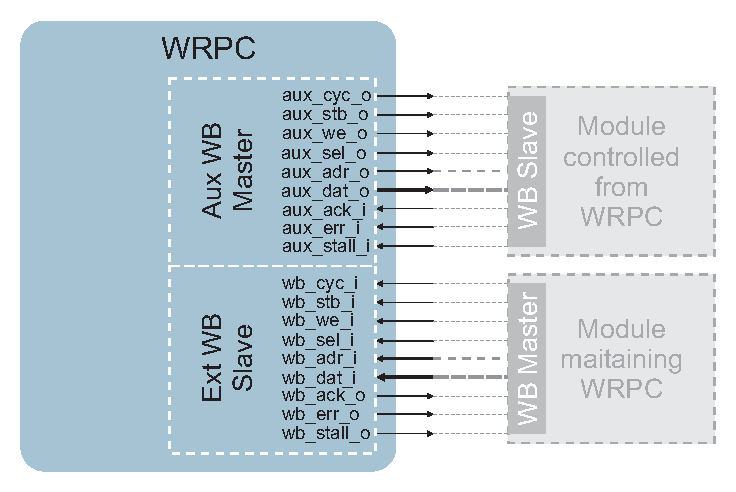
\includegraphics[width=.7\textwidth]{fig/wrpc_wb.pdf}
    \caption{External Wishbone interfaces of WRPC}
  \end{center}
\end{figure}

{\bf Aux WB Master} is a Pipelined Wishbone Master interface. It is connected
through the Wishbone Crossbar inside the White Rabbit PTP Core to the LM32 soft-core
processor (instantiated inside the WRPC). It can optionally be used to control
any user-defined module having a Pipelined Wishbone Slave interface. In that case, the WRPC software
has to be modified to control additional modules connected to the \emph{Aux WB
Master} interface.\\

{\bf Ext WB Slave} is a Wishbone Slave interface that operates in Pipelined or
Classic mode (selected with \emph{g\_interface\_mode} generic), with the address bus
granularity set with \linebreak \emph{g\_address\_granularity} generic. It gives the access
to control all the WRPC internals. In the WRPC reference design it is connected to
the Gennum GN4124 IP-core and used to upload WRPC software to its internal memory.\\

HDL modules accessible through \emph{Ext WB Slave} interface:
\begin{center}
  \begin{tabular}{|l|l|}
    \hline {\bf module name} & {\bf offset (bytes)}\\
    \hline
    WRPC internal memory & 0x00000\\
                Mini NIC & 0x20000\\
                Endpoint & 0x20100\\
                Soft PLL & 0x20200\\
           PPS generator & 0x20300\\
                  Syscon & 0x20400\\
                    UART & 0x20500\\
           1-Wire Master & 0x20600\\
           Aux WB Master & 0x20700\\
    \hline
  \end{tabular}
\end{center}
